% !TEX root = ../main.tex

\chapter{Notas}

\section{Token do BreezoMeter}
É de salientar que possivelmente, na altura de avaliação, o \textit{token} do \textit{BreezoMeter} usado durante o desenvolvimento poderá já não estar ativo. Sendo assim, é possível adicionar um novo \textit{token} no ficheiro \textbf{\textit{application.properties}}, como demonstrado na figura \ref{fig:properties}.

\begin{figure}[h]
   \centering
   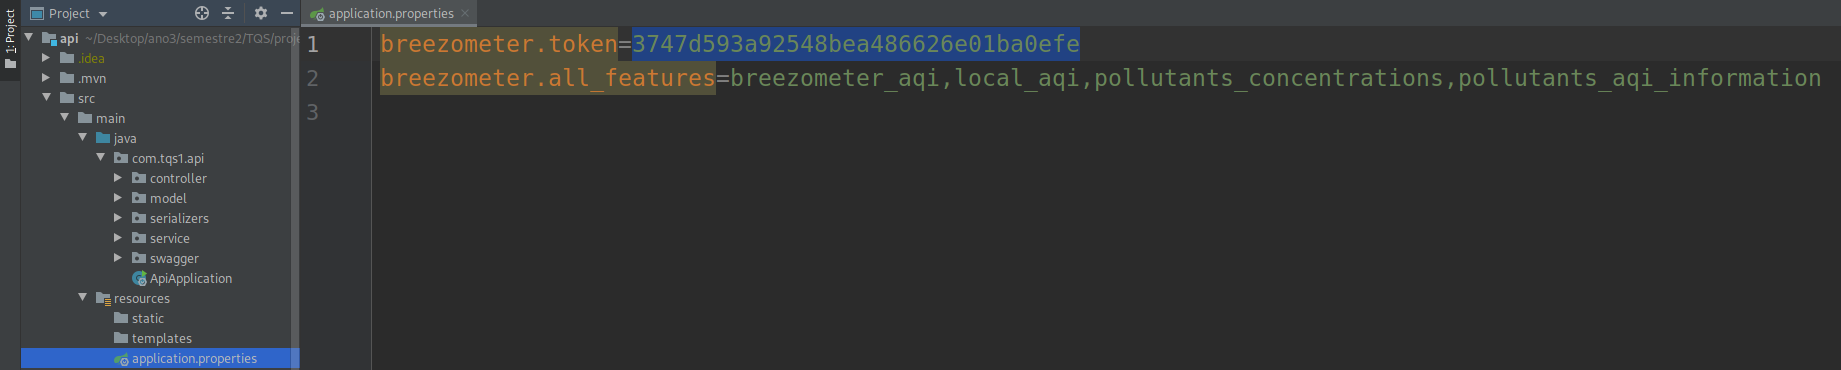
\includegraphics[width=0.90\textwidth]{images/properties}
   \caption{Colocar um novo \textit{token} onde selecionado na imagem.}
   \label{fig:properties}
\end{figure}
